% !TEX root = 03.tex

\section{LLVM framework quick start}


\begin{frame}{Commands}
	\begin{description}[llvm-dwarfdump]
		\item[llvm-as] LLVM assembler
		\item[llvm-dis] LLVM disassembler
		\item[opt] LLVM optimizer
		\item[llc] LLVM static compiler
		\item[lli] directly execute programs from LLVM bitcode
		\item[llvm-link] LLVM bitcode linker
		\item[llvm-mca] LLVM machine code analyzer
		\item[llvm-nm] list LLVM bitcode and object file's symbol table
		\item[llvm-stress] generate random .ll files
		\item[llvm-config] prints out install configuration parameters
		\item[llvm-dwarfdump] print contents of DWARF sections
	\end{description}
	\vfill
	For a complete reference, see the LLVM command guide\footnote{\url{http://llvm.org/docs/CommandGuide/index.html}}
\end{frame}


\begin{frame}{Simulating a LLVM driver manually}
	\noindent\hspace{-1.2cm}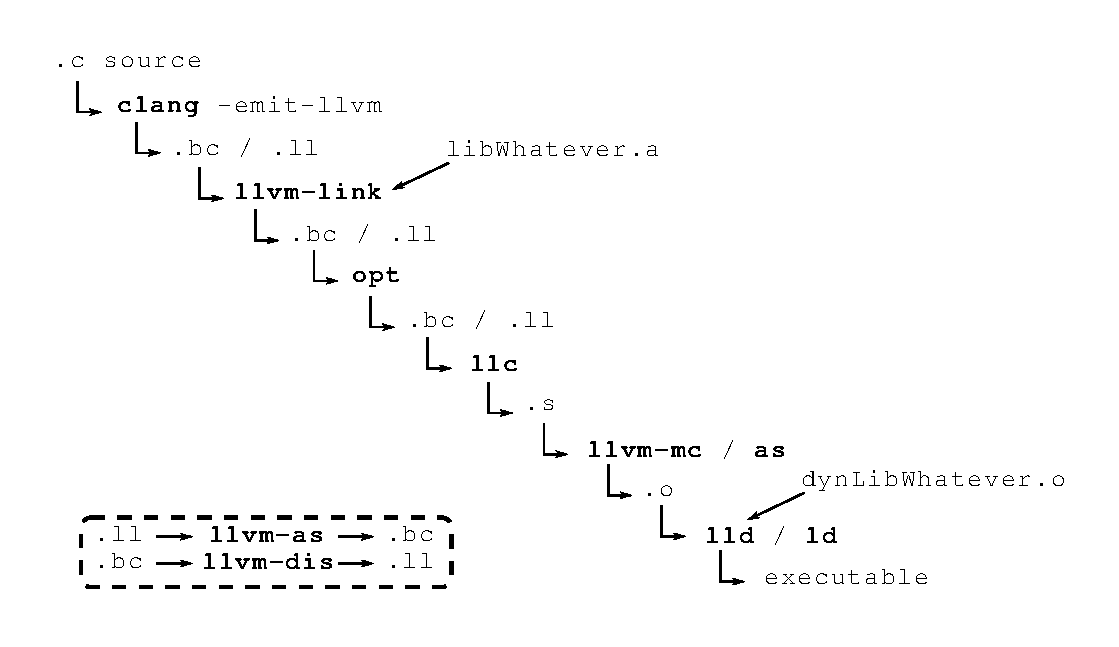
\includegraphics[width=13cm]{img/toolchain}
\end{frame}


\begin{frame}{Writing a LLVM pass}
	There are a lot of tutorials available:
	\vfill
	\begin{itemize}
		\item Official developer guide\\ \href{http://llvm.org/docs/WritingAnLLVMPass.html}{\url{llvm.org/docs/WritingAnLLVMPass}}
		\vfill
		\item Out-of-source pass\\ \href{https://github.com/quarkslab/llvm-dev-meeting-tutorial-2015}{\url{github.com/quarkslab/llvm-dev-meeting-tutorial-2015}}
	\end{itemize}
	\vfill
	We will follow the first one, with a few adjustments.
\end{frame}


\begin{frame}{Testing}
LLVM has an internal testing infrastructure\footnote{\url{http://llvm.org/docs/TestingGuide.html}}.
Please use it.
\\
\begin{description}
	\item[llvm-lit] LLVM Integrated Tester
\end{description}
\begin{enumerate}
	\item Forge a proper LLVM-IR input file (.ll) for your test case
	\item Instrument it with \texttt{lit} script comments
	\item Run \texttt{lit} on your test
		\begin{itemize}
			\item \texttt{llvm-lit ~/llvm/test/myTests/singleTest.ll}\\ run a single test
			\item \texttt{llvm-lit ~/llvm/test/myTests}\\ run the test suite (folder)
		\end{itemize}
	\item Run \texttt{lit} on the LLVM test suite (regression testing)
\end{enumerate}
\vfill
To submit a bug report to LLVM developers you will be asked to write a \texttt{lit} test case that highlights the bug.
\end{frame}
